% =====================================================================
%  Fundamentals of Deep Learning — Class 3 (29 July)
%  Topic (course plan): NN-1
%  Subtopics: Perceptrons; Perceptron Learning Algorithm
%
%  Main source: R. Rojas, Neural Networks (Springer, 1996), Ch. 3-4.
%  Supporting: NPTEL Computational Neuroscience notes (ch6).
%  Figures used with attribution; teaching sequence follows Rojas.
%
%  Compile:  xelatex main.tex   (run twice)
% =====================================================================
\documentclass[aspectratio=169, 11pt]{beamer}

\usetheme{metropoliscustom}

\usepackage{graphicx}
\graphicspath{{Class03_Perceptrons_PLA/figs_official/}{figs_official/}}
\usepackage{amsmath, amssymb}
\usepackage{bm}
\usepackage{tikz}
\usetikzlibrary{arrows.meta, positioning, calc}
\tcbuselibrary{skins}

\definecolor{mpc}{HTML}{341651}    % McCulloch-Pitts side (indigo)
\definecolor{pcc}{HTML}{800000}    % perceptron side (maroon)

% ---- parallel strip: McCulloch-Pitts (left) vs Perceptron (right)
\newcommand{\mppar}[2]{%
  \vfill
  {\footnotesize
  \begin{tcolorbox}[enhanced, sidebyside, sidebyside align=top,
                    lefthand ratio=0.485,
                    segmentation style={mpc!35, line width=0.6pt},
                    colback=mpc!5, colframe=mpc!35, boxrule=0.5pt,
                    arc=1.5mm, left=2mm, right=2mm, top=0.8mm, bottom=0.8mm]
    {\color{mpc}\textbf{M--P}}\;\; #1
  \tcblower
    {\color{pcc}\textbf{PERCEPTRON}}\;\; #2
  \end{tcolorbox}}%
  \vspace{0.6em}%
}

\newcommand{\figsource}[1]{{\scriptsize\color{mcMuted} #1}}

% =====================================================================
\title{Perceptrons and the Perceptron Learning Algorithm}
\subtitle{Weighted threshold units, and how they learn}
\author{Fundamentals of Deep Learning \ \textperiodcentered\ Class 3}
\institute{Prof.~Nirav Bhatt}
\date{29 July}

\footleft{Fundamentals of Deep Learning}
\footright{Perceptrons and the PLA}
\titlelogos{}

\begin{document}

\maketitle

\begin{frame}{Outline}
  \tableofcontents
\end{frame}

% =====================================================================
\section{From Threshold Logic to the Perceptron}
% =====================================================================

\begin{frame}{Where Class 2 left us}
  \begin{itemize}
    \item A McCulloch--Pitts unit fires when
          $x_1+\cdots+x_n \ge \theta$ --- inputs are summed
          with \alert{equal weight}
    \item Geometrically it is a \alert{separating plane}, but
          the planes are always \alert{parallel} (unit
          weights, fixed orientation)
    \item Consequence: many linearly separable functions
          cannot be realised by a \emph{single} M--P unit
          without extra structure
  \end{itemize}
  \vspace{0.3em}
  \begin{redhighlight}
    Give each input its own \alert{weight} and add a
    \alert{bias}: the plane can now take any orientation and
    offset. This is the \alert{perceptron}.
  \end{redhighlight}
\end{frame}

\begin{frame}{A little history: Rosenblatt's perceptron}
  \centering
  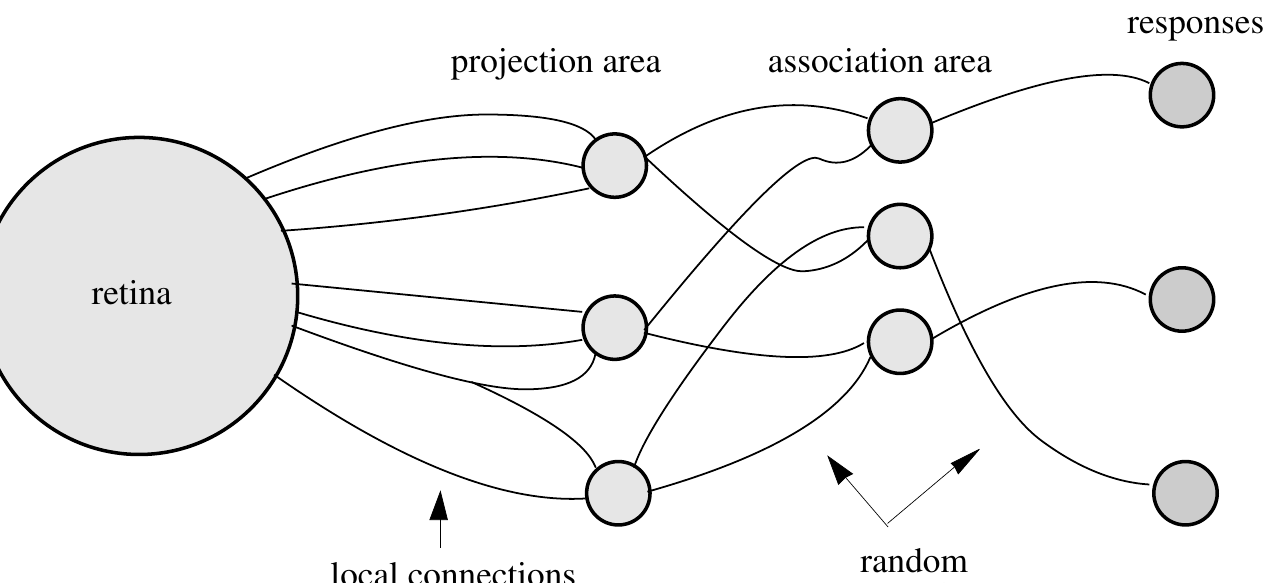
\includegraphics[height=0.30\textheight]{classic_perceptron}
  \\[0.1em]
  \figsource{Rojas (1996), Fig.~3.1: the classical perceptron
  [after Rosenblatt 1958].}
  \vspace{0.1em}
  \begin{itemize}\setlength{\itemsep}{1pt}
    \item Rosenblatt (1958) wired a \alert{retina} of pixels
          to weighted threshold units --- built to
          \alert{learn} to recognise patterns
    \item Its only formal difference from a McCulloch--Pitts
          unit is the presence of \alert{weights}
          \hfill{\scriptsize Rojas (1996), \S3.1}
    \item It drew great excitement --- and, later, a famous
          controversy over its limits
  \end{itemize}
\end{frame}

\begin{frame}{The perceptron: a weighted threshold unit}
  \centering
  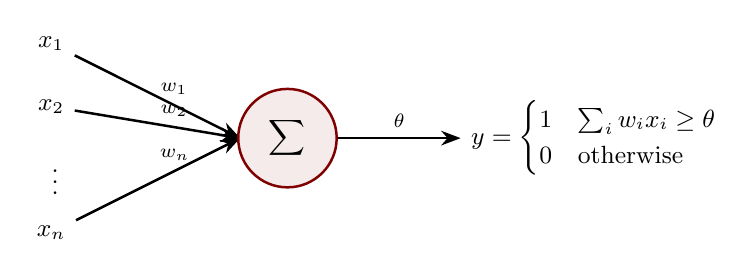
\begin{tikzpicture}[>=Stealth, line width=0.9pt,
      every node/.style={font=\small}]
    \foreach \i/\y in {1/1.4,2/0.6,n/-1.0}{
      \node (x\i) at (0,\y) {$x_{\i}$};
      \draw[->] (x\i) -- node[above, pos=0.6, font=\scriptsize]
        {$w_{\i}$} (2.4,0.2);
    }
    \node at (0.05,-0.25) {$\vdots$};
    \node[circle, draw=pcc, fill=pcc!8, minimum size=1.25cm]
      (sum) at (3.0,0.2) {$\displaystyle\sum$};
    \draw[->] (sum) -- node[above, font=\scriptsize]
      {$\theta$} (5.2,0.2);
    \node[right] at (5.2,0.2)
      {$y=\begin{cases}1 & \sum_i w_i x_i \ge \theta\\
       0 & \text{otherwise}\end{cases}$};
  \end{tikzpicture}
  \vspace{0.6em}
  \begin{itemize}\setlength{\itemsep}{2pt}
    \item Each input $x_i$ carries a real \alert{weight}
          $w_i$; the unit fires if
          $\mathbf{w}\!\cdot\!\mathbf{x}\ge\theta$
    \item Introduced by Rosenblatt (1958); weights make the
          separating plane \alert{freely orientable}
  \end{itemize}
  \mppar{fixed unit weights}{\alert{learnable} real weights}
\end{frame}

\begin{frame}{Weights tilt the separating plane}
  \begin{columns}[T, onlytextwidth]
    \begin{column}{0.5\textwidth}
      \centering
      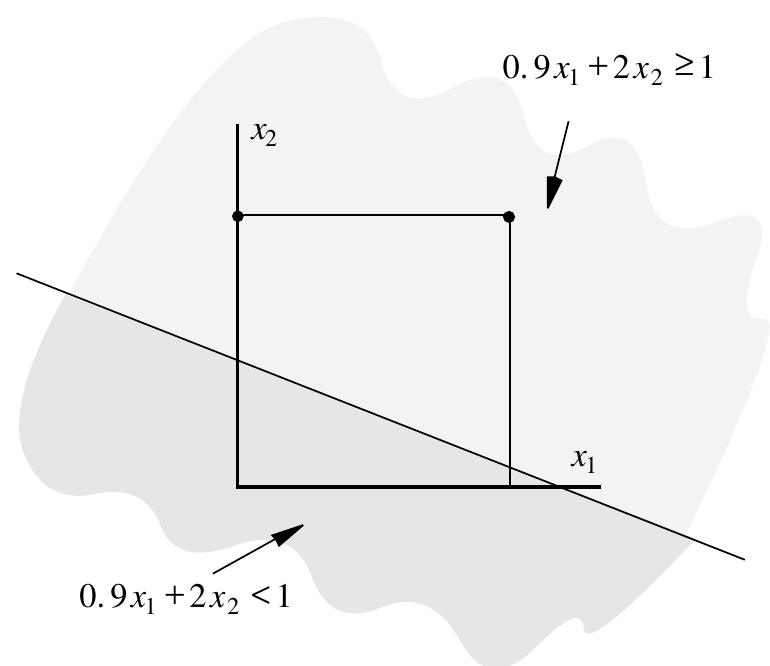
\includegraphics[height=0.46\textheight]{sep_perceptron}
      \\[0.1em]
      \figsource{Rojas (1996), Fig.~3.4.}
    \end{column}
    \hfill
    \begin{column}{0.46\textwidth}
      \vspace{0.3em}
      {\small A perceptron with weights $(0.9, 2)$ and
      threshold $1$ tests $\;0.9\,x_1 + 2\,x_2 \ge 1$:}
      \begin{itemize}\setlength{\itemsep}{2pt}
        \item The boundary is a line of \alert{arbitrary
              slope} --- not just the parallel M--P planes
        \item Any linear separation of the plane can be
              realised by choosing $\mathbf{w},\theta$
      \end{itemize}
    \end{column}
  \end{columns}
  \mppar{parallel planes only}{any orientation and offset}
\end{frame}

\begin{frame}{The bias trick}
  \begin{columns}[T, onlytextwidth]
    \begin{column}{0.52\textwidth}
      \centering
      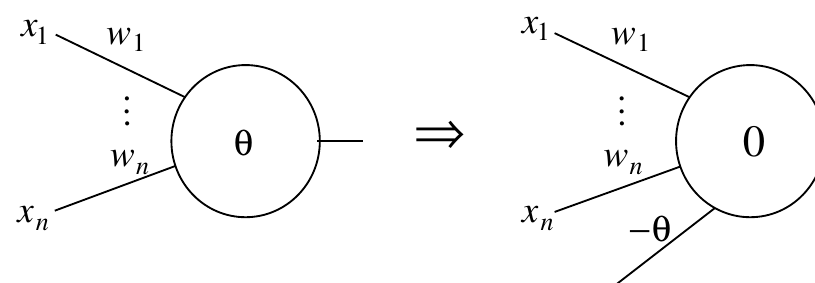
\includegraphics[width=\linewidth]{bias}
      \\[0.1em]
      \figsource{Rojas (1996), Fig.~3.5.}
    \end{column}
    \hfill
    \begin{column}{0.44\textwidth}
      \vspace{0.3em}
      \begin{itemize}\setlength{\itemsep}{2pt}
        \item Fold the threshold into a weight: add an input
              fixed at $1$ with weight $-\theta$
        \item The condition
              $\mathbf{w}\!\cdot\!\mathbf{x}\ge\theta$
              becomes $\tilde{\mathbf{w}}\!\cdot\!
              \tilde{\mathbf{x}}\ge 0$
        \item This $-\theta$ weight is the \alert{bias}; the
              boundary may now miss the origin
      \end{itemize}
    \end{column}
  \end{columns}
  \mppar{threshold $\theta$ compared explicitly}
        {threshold absorbed as a \alert{bias} weight}
\end{frame}

\begin{frame}{Extended input space}
  With the bias folded in, every input becomes an
  \alert{extended vector} and the test is homogeneous:
  \[
    \tilde{\mathbf{x}} = (x_1,\dots,x_n,1),
    \qquad
    \tilde{\mathbf{w}} = (w_1,\dots,w_n,-\theta),
    \qquad
    \tilde{\mathbf{w}}\cdot\tilde{\mathbf{x}} \ge 0.
  \]
  \begin{itemize}\setlength{\itemsep}{1pt}
    \item The separating plane now passes through the
          \alert{origin} of the $(n{+}1)$-dimensional space
    \item Training data split into two sets: $P$ (should
          output $1$) and $N$ (should output $0$)
    \item Goal: find $\tilde{\mathbf{w}}$ with
          $\tilde{\mathbf{w}}\!\cdot\!\mathbf{x}>0$ for all
          $\mathbf{x}\in P$ and $<0$ for all
          $\mathbf{x}\in N$
  \end{itemize}
  \mppar{hand-designed weights}
        {weights to be \alert{found} from labelled data}
\end{frame}

% =====================================================================
\section{Input Space and Weight Space}
% =====================================================================

\begin{frame}{Two dual viewpoints}
  \begin{columns}[T, onlytextwidth]
    \begin{column}{0.5\textwidth}
      \centering
      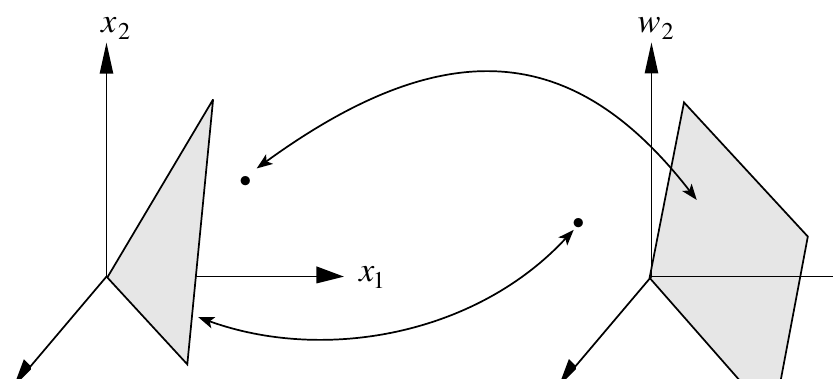
\includegraphics[width=\linewidth]{duality}
      \\[0.1em]
      \figsource{Rojas (1996), Fig.~3.7.}
    \end{column}
    \hfill
    \begin{column}{0.46\textwidth}
      \vspace{0.2em}
      \begin{itemize}\setlength{\itemsep}{1pt}
        \item In \alert{input space}, a fixed
              $\mathbf{w}$ is a plane splitting the inputs
        \item In \alert{weight space}, a fixed input
              $\mathbf{x}$ is a plane splitting the weight
              vectors
        \item $\mathbf{w}\!\cdot\!\mathbf{x}=0$ is symmetric:
              points and planes \alert{swap roles}
      \end{itemize}
    \end{column}
  \end{columns}
  \begin{redhighlight}
    Learning is a search in \alert{weight space} for a point
    on the correct side of every data plane.
  \end{redhighlight}
\end{frame}

% =====================================================================
\section{The Learning Problem}
% =====================================================================

\begin{frame}{What does it mean to `learn'?}
  \centering
  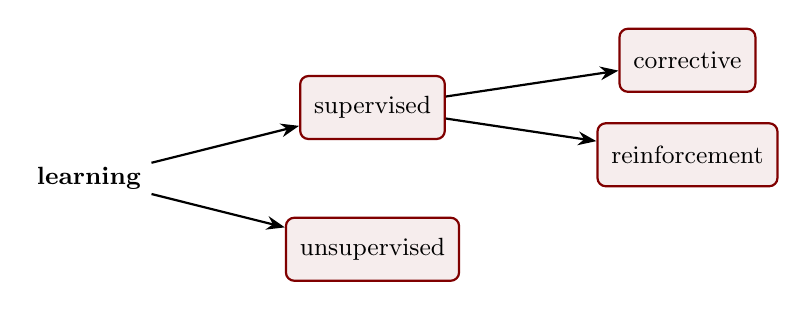
\begin{tikzpicture}[>=Stealth, line width=0.8pt,
      lvl/.style={font=\small},
      leaf/.style={rounded corners=3pt, draw=pcc, fill=pcc!7,
                   font=\small, inner xsep=5pt, minimum height=0.8cm}]
    \node[lvl] (root) at (0,0) {\textbf{learning}};
    \node[leaf] (sup) at (3.6,0.9) {supervised};
    \node[leaf] (uns) at (3.6,-0.9) {unsupervised};
    \node[leaf] (cor) at (7.6,1.5) {corrective};
    \node[leaf] (rei) at (7.6,0.3) {reinforcement};
    \draw[->] (root)--(sup); \draw[->] (root)--(uns);
    \draw[->] (sup)--(cor); \draw[->] (sup)--(rei);
  \end{tikzpicture}
  \vspace{0.5em}
  \begin{itemize}\setlength{\itemsep}{1pt}
    \item \alert{Supervised}: each input comes with a target;
          \alert{unsupervised}: the network finds structure
          on its own
    \item Supervised splits into \alert{corrective} (fix the
          error directly) and \alert{reinforcement} (reward
          or punish)
    \item The \alert{perceptron} rule is supervised with
          error correction
          \hfill{\scriptsize Rojas (1996), \S4.1.1}
  \end{itemize}
\end{frame}

\begin{frame}{Learning as a search for parameters}
  \begin{itemize}
    \item A network is a \alert{parametric system}: fix the
          architecture, and the weights are \alert{free
          parameters} to be set
    \item ``Learning'' means \alert{searching} weight space
          for values that make the outputs match the targets
    \item The search is driven by an \alert{error signal}:
          how wrong the current weights are on the training
          data
    \item Every learning rule in this course is a different
          way of \alert{descending} that error
          \hfill{\scriptsize Rojas (1996), \S4.1}
  \end{itemize}
  \mppar{weights fixed by the designer}
        {weights \alert{searched} to minimise error}
\end{frame}

\begin{frame}{The error surface}
  \begin{columns}[T, onlytextwidth]
    \begin{column}{0.5\textwidth}
      \centering
      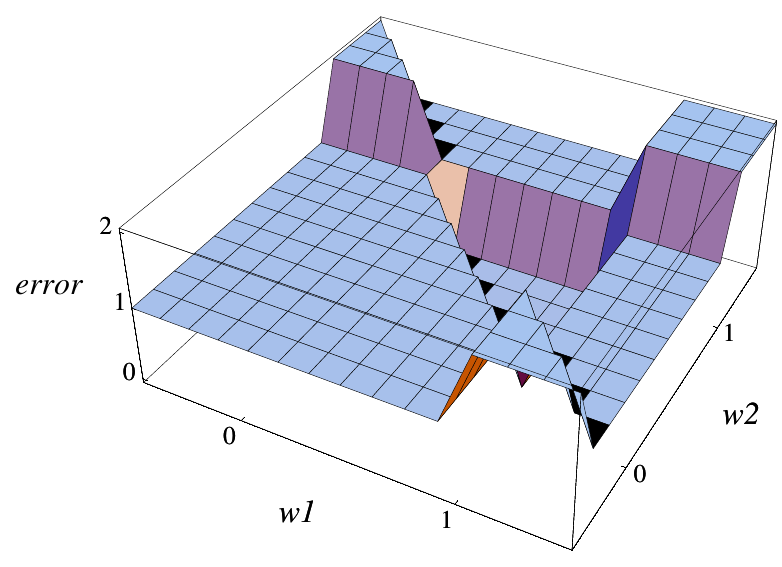
\includegraphics[height=0.46\textheight]{error_surface}
      \\[0.1em]
      \figsource{Rojas (1996), Fig.~4.5: error for AND, over
      weights $(w_1,w_2)$.}
    \end{column}
    \hfill
    \begin{column}{0.46\textwidth}
      \vspace{0.3em}
      \begin{itemize}\setlength{\itemsep}{2pt}
        \item Each point is a weight vector; the height is
              \alert{how many examples it misclassifies}
        \item The flat \alert{valley floor} (error $0$) is the
              \alert{solution region}
        \item Learning $=$ walking downhill to that valley,
              using only \alert{local} decisions
      \end{itemize}
    \end{column}
  \end{columns}
  \mppar{no error to descend --- weights hand-set}
        {descend the error surface to a zero-error region}
\end{frame}

\begin{frame}{Absolute linear separability}
  \begin{itemize}
    \item The PLA needs a \alert{strict} separation: every
          positive example on the \emph{open} positive side,
          every negative on the open negative side
    \item If a separating plane exists, we can always find one
          with a \alert{margin} --- no data point lies exactly
          on it
    \item This \alert{absolute} separability is what the
          convergence proof will rely on
          \hfill{\scriptsize Rojas (1996), \S4.1.3}
  \end{itemize}
  \vspace{0.3em}
  \begin{redhighlight}
    ``Separable'' is not quite enough --- we need a little
    room on each side. Then learning is guaranteed to finish.
  \end{redhighlight}
\end{frame}

% =====================================================================
\section{The Perceptron Learning Algorithm}
% =====================================================================

\begin{frame}{Learning as error correction}
  \begin{itemize}
    \item Start from a random weight vector; present training
          examples one at a time
    \item If the current example is classified
          \alert{correctly}, leave the weights unchanged
    \item If it is \alert{wrong}, nudge the weights toward
          the correct decision --- and repeat
  \end{itemize}
  \vspace{0.3em}
  \begin{redhighlight}
    Only mistakes drive learning. The rule is local, online,
    and strikingly simple.
  \end{redhighlight}
\end{frame}

\begin{frame}{The algorithm}
  Sets $P$ (target $1$) and $N$ (target $0$), extended
  vectors. Seek $\mathbf{w}$ with
  $\mathbf{w}\!\cdot\!\mathbf{x}>0$ on $P$,
  $\mathbf{w}\!\cdot\!\mathbf{x}\le 0$ on $N$
  (Rojas, 1996, \S4.2):
  \vspace{0.2em}
  \begin{tcolorbox}[colback=pcc!4, colframe=pcc!40,
                    boxrule=0.5pt, arc=1mm, left=3mm]
  {\small
  \textbf{start:} random $\mathbf{w}_0$, \; $t:=0$\\[2pt]
  \textbf{test:} pick $\mathbf{x}\in P\cup N$ at random\\
  \quad if correctly classified: go to \textbf{test}\\
  \quad if $\mathbf{x}\in P$ and $\mathbf{w}_t\!\cdot\!\mathbf{x}\le 0$:
        go to \textbf{add}\\
  \quad if $\mathbf{x}\in N$ and $\mathbf{w}_t\!\cdot\!\mathbf{x}\ge 0$:
        go to \textbf{subtract}\\[2pt]
  \textbf{add:} $\mathbf{w}_{t+1}=\mathbf{w}_t+\mathbf{x}$,
        \ $t{:=}t{+}1$; go to \textbf{test}\\[2pt]
  \textbf{subtract:} $\mathbf{w}_{t+1}=\mathbf{w}_t-\mathbf{x}$,
        \ $t{:=}t{+}1$; go to \textbf{test}}
  \end{tcolorbox}
\end{frame}

\begin{frame}{Why the update works}
  \begin{columns}[T, onlytextwidth]
    \begin{column}{0.5\textwidth}
      \centering
      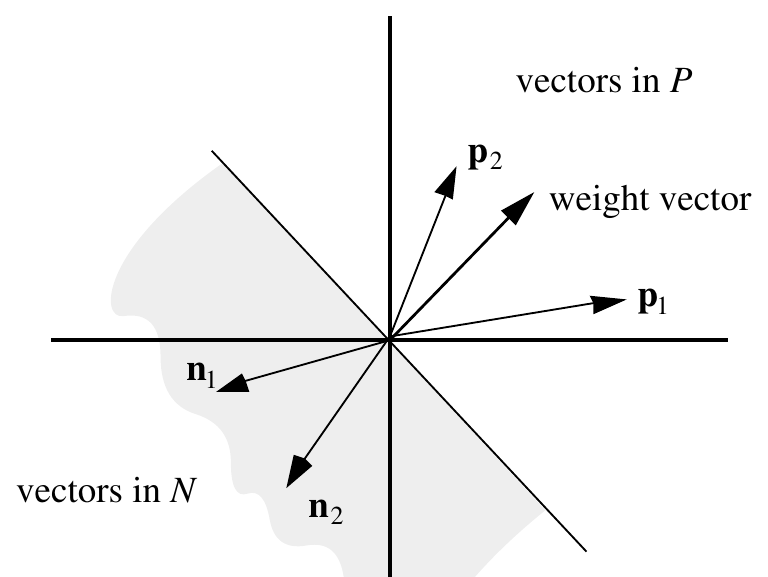
\includegraphics[height=0.42\textheight]{pla_input}
      \\[0.1em]
      \figsource{Rojas (1996), Fig.~4.8.}
    \end{column}
    \hfill
    \begin{column}{0.46\textwidth}
      \vspace{0.2em}
      {\small A misclassified $\mathbf{x}\in P$ has
      $\mathbf{w}\!\cdot\!\mathbf{x}\le 0$. After
      $\mathbf{w}'=\mathbf{w}+\mathbf{x}$:}
      \[
        \mathbf{w}'\!\cdot\!\mathbf{x}
        = \mathbf{w}\!\cdot\!\mathbf{x} + \lVert\mathbf{x}\rVert^2
      \]
      \begin{itemize}\setlength{\itemsep}{1pt}
        \item The dot product \alert{increases} --- the
              weight rotates \emph{toward} $\mathbf{x}$
        \item For $\mathbf{x}\in N$ we subtract, rotating
              \emph{away} --- symmetric fix
      \end{itemize}
    \end{column}
  \end{columns}
  \mppar{no update rule --- weights set by hand}
        {each mistake rotates $\mathbf{w}$ the right way}
\end{frame}

\begin{frame}{The update on the error surface}
  \begin{columns}[T, onlytextwidth]
    \begin{column}{0.56\textwidth}
      \centering
      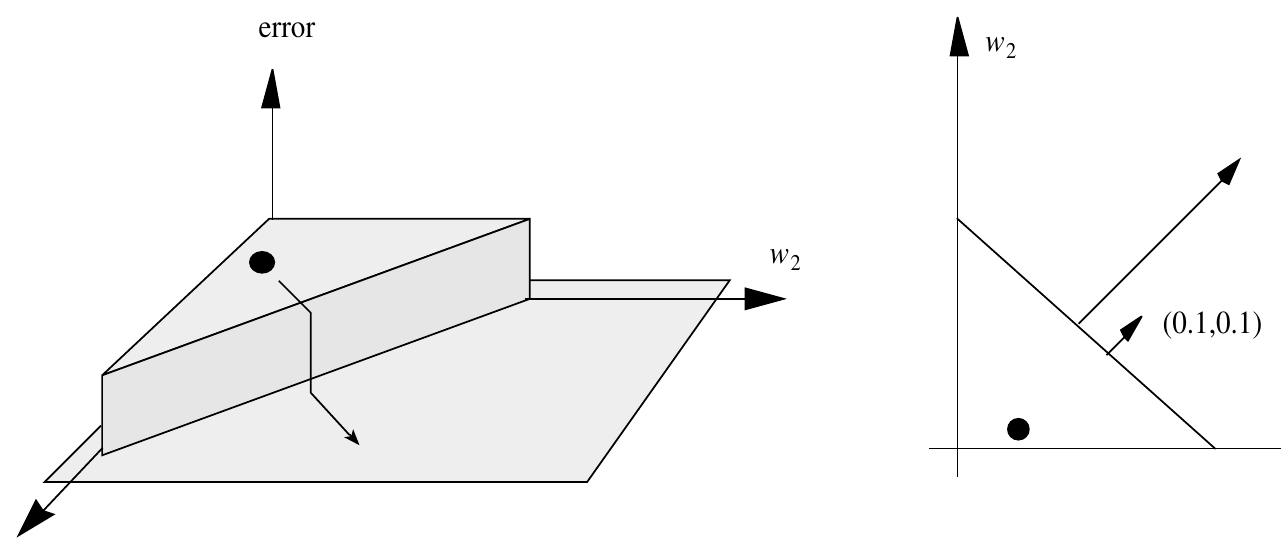
\includegraphics[width=\linewidth]{weight_update}
      \\[0.1em]
      \figsource{Rojas (1996), Fig.~4.11: error surface
      (left) and weight space (right).}
    \end{column}
    \hfill
    \begin{column}{0.40\textwidth}
      \vspace{0.2em}
      \begin{itemize}\setlength{\itemsep}{1pt}
        \item Each correction moves $\mathbf{w}$ into a
              region of \alert{lower error}
        \item In weight space, every misclassified point
              carves off a half-space; the solution is their
              \alert{intersection}
        \item The algorithm walks toward that
              \alert{solution region}
      \end{itemize}
    \end{column}
  \end{columns}
\end{frame}

\begin{frame}{Fixing the error in one step}
  The plain rule nudges; we can instead \alert{fully correct}
  a mistake. For $\mathbf{x}\in P$ with
  $\mathbf{w}\!\cdot\!\mathbf{x} = -\delta \le 0$, set
  (Rojas, 1996, \S4.2.3):
  \[
    \mathbf{w}' = \mathbf{w}
    + \frac{\delta + \varepsilon}{\lVert\mathbf{x}\rVert^2}\,
    \mathbf{x}
    \quad\Rightarrow\quad
    \mathbf{w}'\!\cdot\!\mathbf{x} = \varepsilon > 0.
  \]
  \begin{itemize}\setlength{\itemsep}{1pt}
    \item One update moves $\mathbf{x}$ just past the boundary
          (by a margin $\varepsilon$) --- the mistake is
          \alert{fixed immediately}
    \item Making $\varepsilon$ small avoids overshooting into
          a worse region
    \item This \alert{corrective} variant learns faster than
          the plain add/subtract rule
  \end{itemize}
  \mppar{no notion of correction}
        {each step \alert{eliminates} one error outright}
\end{frame}

% =====================================================================
\section{Convergence and Limits}
% =====================================================================

\begin{frame}{The perceptron convergence theorem}
  \begin{redhighlight}
    If $P$ and $N$ are \alert{linearly separable}, the
    perceptron learning algorithm makes only a
    \alert{finite} number of weight updates --- it converges
    to a separating $\mathbf{w}$ in finite time.
  \end{redhighlight}
  \vspace{0.4em}
  \begin{itemize}\setlength{\itemsep}{2pt}
    \item Idea of the proof: if a solution
          $\mathbf{w}^{*}$ exists, each update increases the
          alignment $\mathbf{w}\!\cdot\!\mathbf{w}^{*}$ faster
          than it grows $\lVert\mathbf{w}\rVert$
    \item Bounding the two quantities forces the number of
          updates to be finite
          \hfill{\scriptsize Rojas (1996), \S4.2--4.3}
    \item Guarantee of \alert{existence and termination} ---
          not of speed
  \end{itemize}
\end{frame}

\begin{frame}{How long can it take? Worst case}
  \begin{columns}[T, onlytextwidth]
    \begin{column}{0.42\textwidth}
      \centering
      \begin{tikzpicture}[line width=0.9pt, scale=0.72]
        \fill[mpc!12] (-1.4,-1.4) -- (1.0,1.4) -- (-1.4,1.4) -- cycle;
        \fill[pcc!12] (1.4,1.4) -- (-1.0,-1.4) -- (1.4,-1.4) -- cycle;
        \draw[mpc, thick] (-1.2,-1.4) -- (0.9,1.4);
        \draw[pcc, thick] (-0.9,-1.4) -- (1.2,1.4);
        \foreach \p in {(-1.1,0.6),(-0.9,-0.3),(-1.2,-0.9),(-0.6,1.0)}
          \node[mpc, font=\scriptsize] at \p {$\circ$};
        \foreach \p in {(1.1,-0.5),(0.9,0.4),(1.2,1.0),(0.6,-1.0)}
          \node[pcc, font=\scriptsize] at \p {$\times$};
        \draw[<->, mcMuted] (-0.15,0) -- (0.15,0);
        \node[mcMuted, font=\scriptsize] at (0,-0.4) {margin};
      \end{tikzpicture}
      \\[0.1em]
      \figsource{cf.\ Rojas (1996), \S4.2.5.}
    \end{column}
    \hfill
    \begin{column}{0.54\textwidth}
      \vspace{0.2em}
      \begin{itemize}\setlength{\itemsep}{1pt}
        \item Convergence is guaranteed, but the step count
              can be \alert{large}
        \item A \alert{thin margin} means the weight vector
              must be nudged many times --- updates grow with
              the \alert{inverse squared margin}
        \item Still \alert{finite}: the theorem holds, only
              the speed suffers
      \end{itemize}
    \end{column}
  \end{columns}
  \mppar{no learning --- nothing to time}
        {finite, but slow when the margin is thin}
\end{frame}

\begin{frame}{The limit: XOR and non-separable data}
  \begin{columns}[T, onlytextwidth]
    \begin{column}{0.4\textwidth}
      \centering
      \begin{tikzpicture}[line width=0.9pt, scale=1.5]
        \draw[->] (-0.2,0) -- (1.35,0) node[right,font=\scriptsize]{$x_1$};
        \draw[->] (0,-0.2) -- (0,1.35) node[above,font=\scriptsize]{$x_2$};
        \node[circle, draw=mpc, fill=mpc!15, minimum size=4pt,
              inner sep=1.2pt] at (0,0) {};
        \node[circle, draw=mpc, fill=mpc!15, minimum size=4pt,
              inner sep=1.2pt] at (1,1) {};
        \node[pcc, font=\small] at (0,1) {$\bm\times$};
        \node[pcc, font=\small] at (1,0) {$\bm\times$};
        \draw[mcMuted, dashed] (-0.12,0.6) -- (1.15,0.72);
        \draw[mcMuted, dashed] (0.4,-0.12) -- (0.62,1.2);
      \end{tikzpicture}
      \\[0.1em]
      \figsource{$\bm\times$: XOR $=1$; \; $\circ$: XOR $=0$.}
    \end{column}
    \hfill
    \begin{column}{0.55\textwidth}
      \begin{itemize}\setlength{\itemsep}{1pt}
        \item A single perceptron computes exactly the
              \alert{linearly separable} functions --- any
              orientation, but still one line
        \item \alert{XOR} is not separable: no line puts both
              $\times$ on one side and both $\circ$ on the
              other
        \item On non-separable data the PLA \alert{never
              terminates}; the \alert{pocket algorithm} keeps
              the best weights seen
              \hfill{\scriptsize Rojas, \S4.2.4}
      \end{itemize}
    \end{column}
  \end{columns}
  \begin{redhighlight}
    One layer is still a linear classifier. XOR needs a
    \alert{hidden layer} --- the shallow network (Classes
    5--7).
  \end{redhighlight}
\end{frame}

\begin{frame}{Takeaways}
  \begin{enumerate}\setlength{\itemsep}{2pt}
    \item A \alert{perceptron} is a threshold unit with
          \alert{learnable weights} and a \alert{bias} ---
          its boundary is a freely oriented hyperplane
    \item The bias trick makes the test homogeneous:
          $\tilde{\mathbf{w}}\!\cdot\!\tilde{\mathbf{x}}\ge 0$
    \item The \alert{PLA} corrects only on mistakes:
          add $\mathbf{x}$ for a missed positive, subtract
          for a missed negative
    \item It \alert{provably converges} when the data are
          linearly separable --- but XOR and non-separable
          sets remain out of reach
  \end{enumerate}
  \vspace{0.3em}
  \begin{redhighlight}
    Class~5: stack weighted units into layers --- the shallow
    neural network.
  \end{redhighlight}
\end{frame}

\begin{frame}{References}
  \footnotesize
  \begin{itemize}
    \item R.~Rojas. \textit{Neural Networks: A Systematic
          Introduction.} Springer, 1996. Chapters 3--4.
          Figures 3.4, 3.5, 3.7, 4.8, 4.11 reproduced with
          attribution.
    \item F.~Rosenblatt (1958). ``The perceptron: a
          probabilistic model for information storage and
          organization in the brain.'' \textit{Psychological
          Review}, 65(6), 386--408.
    \item NPTEL Computational Neuroscience notes
          (perceptrons and MLPs), used for supporting
          intuition.
  \end{itemize}
\end{frame}

\begin{frame}[standout]
  Questions?
\end{frame}

\end{document}
